
\paragraph{Lower body}



\begin{figure}[h!]% order of placement preference: here, top, bottom
\centering
 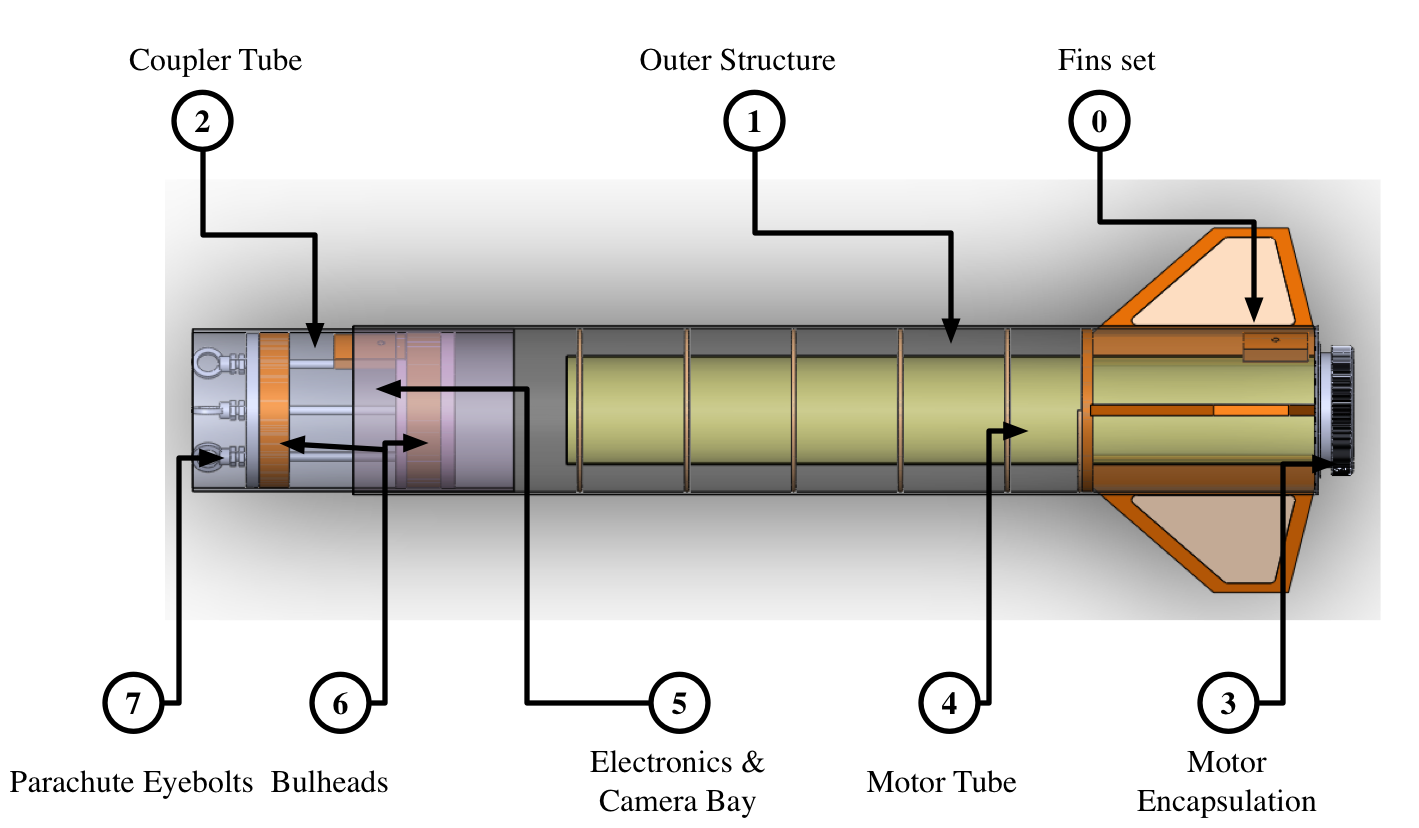
\includegraphics[width=0.8\textwidth]{images/PartsOfRocket}
 \caption{Lower body Main Components}
 \label{f:lower_body}
\end{figure}



\begin{enumerate}
\item Fins Set

Description:

\item Outer Structure

Description: 

Phenolic tube (temperature resistant) bought
\item Coupler tube

Description

\item Motor encapsulation

Description

\item Motor Tube

Description

\item Electronics and Camera Bay

Description:

\item Bulkheads 

- 250  3 layers of Carbon fibre on each side. 15 mm thick

\item Parachute Eyebolts



\end{enumerate}
Coupler Tube


Put the carbon fibre (two layers) without vacuum. 
Bulkhead inside the coupler tube.  3 x M8 rods and one in the centre. 


Holes for airventing


2 x M6 holes with a wood nut to mount the 2 x launch rails (take picture from Oliver) that are on the same part of rocket (on the lower body)



Apply epoxy on the inside, apply on the bulkhead and put them in. 



What to improve: 
- too many airventing holes, maybe we can make them smaller. holes are M5 x 6 => M3 x 6
- the bulkheads


\subsubsection{Upper body}

\subsubsection{Nosecose}